\documentclass{llncs}
\usepackage{amssymb}
\usepackage{amsmath}
\usepackage{views}
\usepackage{graphicx}
\usepackage{xcolor}
\usepackage{UTPCalc}
\usepackage{listings}
\usepackage{PML}
%\usepackage{mathpartir}
\usepackage{epstopdf}
\usepackage{hyperref}
\allowdisplaybreaks[2]
\newif\ifColour
%\Colourtrue
\ifColour
\usepackage{clstlhs}
\else
\usepackage{lstlhs}
\fi
% ----------------------------------------------------------------


\newif\ifDraft
%\Drafttrue  % comment out to turn off note/draft-mode
\ifDraft
  \def\NOTE#1{\textbf{Note: }\textsl{#1}}
  \def\DRAFT#1{\textbf{[Draft: }\textsc{#1}\textbf{]}}
\else
  \def\NOTE#1{}
  \def\DRAFT#1{}
\fi

\title{UTCP: compositional semantics for shared-variable concurrency}%
\author{
Andrew Butterfield
\thanks{%
This work was supported, in part,
by Science Foundation Ireland grants 10/CE/I1855 and
to Lero - the Irish Software Engineering Research Centre (www.lero.ie)}%
}
\institute{
Trinity College Dublin
}
\date{\today}%

\mathchardef\spot="320F
\mathcode`\@=\spot
\mathcode`\|=\mid


\def\lhsDL{\DL(P)}
\def\rhsDL{P \land \setof{in|g|out}}
\def\lblDL{DL-def}

\def\lhsLE{\LE(P)}
\def\rhsLE{P \land [in|g|out]}
\def\lblLE{EL-def}

\def\lhsWWW{\WWW(P)}
\def\rhsWWW{\bigvee_{i \in \Nat} P^i}
\def\lblWWW{WWW-as-NDC}

\def\lhsW{\W(P)}
\def\rhsW{\DL(\LE(\WWW(P)))}
\def\lblW{W-def}

\def\lhsA{A(E|a|N)}
\def\rhsA{E \subseteq ls \land a \land ls'=(ls\setminus E) \cup N}
\def\lblA{A-def}

\def\lhsCA{\catom a}
\def\rhsCA{\W(A(in|a|out))) }
\def\lblCA{sem:atomic}

\def\lhsSEQ{P \cseq Q}
\def\rhsSEQ{\W(P[g_{:1},\ell_g/g,out] \lor Q[g_{:2},\ell_g/g,in])}
\def\lblSEQ{sem:seq}
%   P \cseq Q
%   &\defs&
%   \W(P[g_{:1},\ell_g/g,out] \lor Q[g_{:2},\ell_g/g,in])
%   & \elabel{sem:seq}
%}
%

\def\leftW{\W(~}
\def\phW{\phantom{\leftW}}
\def\rghtW{~)}

\def\lhsPAR{P \parallel Q}
\def\rhsaPAR{A(in|ii|\ell_{g1},\ell_{g2})}
\def\rhsbPAR{P[g_{1::},\ell_{g1},\ell_{g1:}/g,in,out]}
\def\rhscPAR{Q[g_{2::},\ell_{g2},\ell_{g2:}/g,in,out]}
\def\rhsdPAR{A(\ell_{g1:},\ell_{g2:}|ii|out)}
\def\lblPAR{sem:par}

\def\lhsNDC{P+Q}
\def\invNDC{[\g1|\g2]}
\def\rhsNDC{\W(~P[g_{1}/g] \lor Q[g_{2}/g]~)}
\def\lblNDC{sem:NDC}

\def\lhsSTAR{P^*}
\def\rhsaSTAR{A(in|ii|\ell_g)}
\def\rhsbSTAR{A(\ell_g|ii|\ell_{g:})}
\def\rhscSTAR{A(\ell_g|ii|out)}
\def\rhsdSTAR{P[\g{::},\ell_{g:},\ell_g/g,in,out]}
\def\lblSTAR{sem:star}

\def\lhsCND{P \dcond c Q}
\def\invCND{[\ell_{g1}|\g{1:}|\ell_{g2}|\g{2:}]}
\def\rhsaCND{A(in|c \land ii|\ell_{g1})}
\def\rhsbCND{A(in|\lnot c \land ii|\ell_{g2})}
\def\rhscCND{P[\g{1:},\ell_{g1}/g,in]}
\def\rhsdCND{Q[\g{2:},\ell_{g2}/g,in]}
\def\lblCND{sem:cond}

\def\lhsITER{c \ddo P}
\def\rhsaITER{A(in|ii|\ell_g)}
\def\rhsbITER{A(\ell_g|\lnot c \land ii|out)}
\def\rhscITER{A(\ell_g|c \land ii|\ell_{g:}) }
\def\rhsdITER{P[\g{::},\ell_{g:},\ell_g/g,in,out]}
\def\lblITER{sem:iter}


\begin{document}

\maketitle

\begin{abstract}
We present a Unifying Theories of Programming (UTP) semantics
of shared variable concurrency
that is fully compositional.
Previous work was based on mapping such programs,
using labelling of decision points and atomic actions,
to action systems,
which themselves were provided with a UTP semantics.
The translation to action systems was largely compositional,
but their dynamic semantics was based on having all the actions collected together.
Here we take a more direct approach, albeit inspired by the action-systems view,
based on an abstract notion of label generation,
that then exploits the standard use of substitution in UTP,
to obtain a fully compositional semantics.
\end{abstract}

%\newpage % to allow figures on top of first page below during drafting

\section{Introduction}\label{sec:intro}

We now give a proper presentation of our UTP theory
of concurrent programming, looking at both the condition-free command language
of the Views paper\cite{conf/popl/Dinsdale-YoungBGPY13},
as well as the more complete language covered in the UTPP paper\cite{DBLP:conf/icfem/WoodcockH02}.
in UTP.

All references in bold to things
like \textbf{Definition 9} or \textbf{Parameter E} refer to corresponding material
in the Views paper.
The generic definitions from\cite{conf/popl/Dinsdale-YoungBGPY13}
are in Appendix \ref{sec:viewdefs}.

\subsection{The Language Menagerie}

Both languages are concurrent with shared state.
The most abstract is the Command language from \cite{conf/popl/Dinsdale-YoungBGPY13}:
\[
 C ::= a \mid \cskip \mid C \cseq C \mid C \parallel C \mid C+C \mid C^*
\]
with non-deterministic choice and iteration.
Note that we have replaced 
The language from \cite{DBLP:conf/icfem/WoodcockH02} replaces both
non-deterministic constructs by deterministic ones depending
on a condition over shared-state:
\[
 D ::= a \mid \cskip \mid D \cseq D \mid D \parallel D \mid D \dcond c D \mid c \ddo D
\]
We will also consider Process Modelling Language (PML)\cite{DBLP:journals/infsof/AtkinsonWN07}
which is like the Views command language except that atomic actions
have a state-based guard:
\[
 M ::= c \pgrd a \mid \cskip \mid M \cseq M \mid M \parallel M \mid M+M \mid M^*
\]
A key point to note is that the semantics of common constructs is the same
in every language.
Given this observation we shall define a single semantics over
a universal concurrent programming language:
\[
 P ::= c \pgrd a \mid \cskip \mid P \cseq P  \mid P \parallel P
   \mid P+P\mid P^*
   \mid P \dcond c P \mid c \ddo P
\]
where $a$ is simply $\true\pgrd a$.

\section{Labels}\label{sec:labels}

\subsection{Overview}


Concurrent programs are a mix of control constructs ($\cseq,\parallel,+,\dots$)
and atomic actions $a$ that modify \emph{program state} $s$.
This is all that is visible to the programmer.



Our denotational UTP semantics
is inspired by that done for UTPP\cite{DBLP:conf/icfem/WoodcockH02},
itself based on a UTP theory of \emph{action systems}.
In UTPP a new state component, not visible in the program text,
was added: a set of labels ($ls$).
These labels are used to orchestrate the flow of control.
Given an atomic action $a$ that only knows about program state $s$,
we use notation $\catom a$ to describe a lifted version
of $a$ that takes account of the contents of the label-set $ls$.
In effect a lifted atomic state action is disabled until
a particular label is present in that set.
A disabled action does not modify the state any way
and simply monitors the label-set.
Once an action observes the presence/arrival of its label,
it then becomes active.
An active lifted action $\catom a$ atomically modifies the extended state as follows:
\begin{itemize}
  \item It makes the changes to $s$ as determined by its underlying action $a$.
  \item It removes the enabling label from the label-set.
  \item It adds in appropriate ``continuation'' labels to $ls$.
\end{itemize}
In \cite{DBLP:conf/icfem/WoodcockH02},
the language syntax required explicit (starting) labels
for every atomic state change action,
and these are used as lifted action enablers.
The continuation labels were taken to the the enabling labels
of whatever other actions occurred immediately after, in the program.
This means that the resulting semantics is not compositional.

The approach we adopt here is to adopt the notion of \emph{label generators}
to create the labels, so ensuring they are unique,
but in such a way as make the generation a compositional process.
In addition we explicitly associate two labels with every program construct:
one that marks the entry into the construct,
and another that indicates the exit.
In our UTP theory we will introduce two static observation variables,
$in$ and $out$ to record respectively the entry and exit labels
for a given construct.


\subsection{Label Generation}

We want to have a way to associate unique labels
with every atomic action, including those added to manage flow of control,
in a compositional manner.
We start by assuming that we have types for labels,
and label generators:
\RLEQNS{
   l &\in& Lbl
\\ g &\in& Gen
}
We have two distinct things we can do with label generators:
\begin{enumerate}
  \item
   Use it then generate a label,
   in which case we also need to get a transformed generator
   that is guaranteed to never produce the label just generated.
   \RLEQNS{
     new &:&  Gen \fun (Lbl \times Gen)
     & \elabel{new-sig}
   }
  \item
   Split generators into two new generators,
   each of which will produce disjoint sets of labels.
   \RLEQNS{
     split &:& Gen \fun (Gen \times Gen)
     & \elabel{split-sig}
   }
\end{enumerate}
Given $new$ and $split$ above, we can defined a function $labs$ that
returns all the labels produced by a generator,
and express our label uniqueness guarantees.
Assuming that $ (l,g') = new(g)$ and $(g_1,g_2) = split(g)$
we get:
\RLEQNS{
   labs &:& Gen \fun \power Lbl & \elabel{labs-sig}
\\ labs(g)
   &\defs&
   \setof l \cup labs(g')
   \cup
   labs(g_1) \cup labs(g_2) &\ecite{labs-def}
\\ l &\notin& labs(g') &\ecite{new-disj}
\\ labs(g_1) \cap labs(g_2) &=&  \emptyset & \ecite{split-disj}
}

Given the notion of label generators as just described,
we are faced with two problems.
The first is that the notation is quite clumsy:
For example in the semantics to be presented below,
we will need the following generator expression:
$
\pi_2(new(\pi_2(new(\pi_2(split(g))))))
$,
where $\pi_i$ projects out the $i$th element of a pair.
The second is that our definitions above are axiomatic,
and we need to demonstrate some form of model that satisfies
the above laws (\ecite{new-disj},\ecite{split-disj}).
Ideally this should also avoid some sort of global check for uniqueness,
to ensure compositionality of the resulting semantics.

Fortunately,
it turns out there is a shorthand notation that dramatically shortens
generator and label expressions,
while also providing a compositional model that satisfies the laws above.

\subsubsection{Generator Notation}

The idea is to realise that we really have four functions of interest:
\RLEQNS{
   \pi_1 \circ new &:& Gen \fun Lbl
\\ \pi_2 \circ new &:& Gen \fun Gen
\\ \pi_1 \circ split &:& Gen \fun Gen
\\ \pi_2 \circ split &:& Gen \fun Gen
}
For the first one, we shall define a prefix operator $\ell : Gen \fun Lbl$
and render its generator argument as a subscript:
\RLEQNS{
  \ell_g &\defs& \pi_1(new(g)) & \elabel{ell-def}
}

For the other three, we turn them into single-character postfix operators,
themselves being rendered as subscripts:
\RLEQNS{
   \g{:} &\defs& \pi_2 \circ new & \elabel{new-:-def}
\\ \g1   &\defs& \pi_1 \circ split & \elabel{split-1-def}
\\ \g2   &\defs& \pi_2 \circ split & \elabel{split-2-def}
}
We then introduce a notation of generator and label expressions
with the following syntax:
\RLEQNS{
   G \in Gen &::=&  g     & \mbox{the ``root'' generator}
\\           &\mid& G_{:} & \mbox{resulting generator after label produced}
\\           &\mid& G_1   & \mbox{first generator after generator split}
\\           &\mid& G_2   & \mbox{second generator after generator split}
\\ L \in Lbl &::=& \ell_G & \mbox{label produced by generator}
}
Note that our generator expression language has only one variable, $g$,
which denotes the ``root'' generator.
We say the  ``root'' generator because this notion is local to a
particular context, and we can relativise things by replacing $g$
by an appropriate $G$ expression.
We can now revisit our definition of $labs$ and our disjointness rules
with the new notation:
\RLEQNS{
   labs &:& Gen \fun \power Lbl
\\ labs(G) &=& \setof{\ell_G} \cup labs(G_{:}) \cup labs(G_1) \cup labs(G_2)
  &\elabel{labs-def}
\\ \ell_G &\notin& labs(G_{:})
   &\elabel{new-disj}
\\ \emptyset &=& labs(G_1) \cap labs(G_2)
  &\elabel{split-disj}
}
The our complicated example shown earlier:
\[
\pi_2(new(\pi_2(new(\pi_2(split(g))))))
\]
now reduces to
\[
  \g{2::}
\]
If we generate a label with this generator,
then we simplify from
\[
\pi_1(new(\pi_2(new(\pi_2(new(\pi_2(split(g))))))))
\]
to
\[
  \ell_{g2::}
\]

We can also introduce a graphical way to visualise
generators that proves useful as a way to understand
the semantic definitions that occur later on,
as shown in Fig. \ref{fig:new-and-split}
\begin{figure}%
  \centering
  \parbox{1.2in}{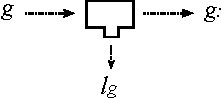
\includegraphics{images/new-label}}%
  \qquad\qquad
  \begin{minipage}{1.2in}%
    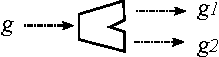
\includegraphics{images/split-gen}
  \end{minipage}%
  \caption{Graphical renderings of $new$ (left) and $split$ (right)}%
  \label{fig:new-and-split}%
\end{figure}



\subsubsection{Model for $new$ and $split$}

The conceptually simplest model of such generators
is one where labels produced are simply the strings of $:$, $1$ and $2$
that designate how the generator was produced from the original root.
For full clarity we show the model here using the full notation.
Both generators and labels are now represented as sequences of the three symbols
$:$, $1$ and $2$.
\RLEQNS{
  s \in LblSym &=& \setof{\texttt{:},\texttt{1},\texttt{2}}
\\ g \in GenSym &=& LblSym^*
\\ l \in Label &=& LblSym^*
\\ new(g) &\defs&  (g,g \cat \seqof{\texttt{:}})
\\ split(g) &\defs&  (g \cat \seqof{\texttt{1}},g \cat \seqof{\texttt{2}})
}
With this model we also get the following law:
For any generator expression $G$,
the following four sets are mutually disjoint:
\[
  \setof{\ell_G}
  \quad
  labs(G_{:})
  \quad
  labs(G_1)
  \quad
  labs(G_2)
  \qquad
  \elabel{labs-fully-disjoint}
\]
This is stronger than we require, but this is not a problem.
We also get three very significant benefits from this model/notation:
\begin{enumerate}
  \item
    It is very easy to decide if two generator expressions
    denote the same label---they do if and only if the expressions are the
    same, which in shorthand terms means the label sequences are the same.
  \item
    It is almost as easy to decide if two generator expressions produce
    disjoint labels.
    This occurs if and only if neither of the sequences of postfix operators
    involved are a prefix of the other.
    Or put differently, a generator's labels are a subset of another's
    iff its postfix sequence extends that of the other generator:
    \RLEQNS{
       labs(\g{\rho}) \subseteq labs(\g{\varrho}) &\equiv& \varrho \leq \rho
       & \elabel{prefix-lab-subset}
    }
    where $\leq$ is the sequence prefix relation.
  \item
    We refer to $g$ as the ``root'' in double quotes,
    because $g$ is not privileged in any way.
    If we substitute a different expression $G$ for $g$
    in the semantics of a construct,
    the behaviour is unchanged.
    In effect $g$ is like a ``base address'',
    with all the labels generated from $g$ being relative to it,
    and replacing $g$ by $G$ simply relocates it and the labels it generates.
    This is the basic mechanism used to construct the semantics
    of all the composite constructs in the language.
\end{enumerate}


\subsection{Label-Set Invariants}

The semantics we propose here depends on the careful management
of when specific labels are, or are not,
present in the global label-set $ls$.
We are looking at a situation where the semantics of any construct
requires associating unique labels with its entry and exit points,
as well as having a label generator provided for use with any sub-components
it might have.

So, from the perspective of any well-program $P$,
we have the following three (static) observation variables.
\RLEQNS{
   in, out &:& Lbl
\\ g &:& Gen
}
Key to the success of this semantics is a collection of label-set invariants
which characterise proper label-set contents,
which are preserved by all label-set manipulations performed
by our semantic definitions.

\subsubsection{Disjoint Labels (DL)}\label{sssec:disjoint-labels}

The first invariant we have is simply one that asserts,
for every construct, that $in$, $out$ and the labels of $g$
are all different
\footnote{The theory can be developed using only $g$ as a static observation,
and letting $\ell_g$ and $\ell_{g:}$ play the role of $in$ and $out$
respectively, in which case Disjoint Labels is automatically satisfied.
However, while this results in an entirely equivalent theory,
it is notationally much more obscure
with definitions and results that are harder to interpret and check.
}%
\RLEQNS{
   in \neq out &\land& \setof{in,out} \cap labs(g) = \emptyset
   & \ecite{Disjoint-Labels}
}



\subsubsection{Label Exclusivity (LE)}\label{sssec:label-exclusivity}

In addition to Disjoint Labels above,
which merely ensures distinctness of labels themselves,
we also need stronger invariants regarding which labels can, or cannot,
occur in the global label set at any one time.
There is not one such Label Exclusivity invariant,
but rather we have that each language construct defines it own
variation, in order to ensure that flow of control is correctly managed.

There is a general version of the invariant, as follows:
\RLEQNS{
   &&
   in \in  ls \implies (\setof{out} \cup labs(g))\cap ls = \emptyset
\\ &\land&
   (labs(g) \cap  ls \neq \emptyset) \implies \setof{in,out}\cap ls = \emptyset
\\ &\land&
   out \in ls \implies (\setof{in} \cup labs(g))\cap ls = \emptyset
   & \ecite{Exclusive-Labels}
}

We also more specific invariants, specific to each composite language construct.
We start with one of the simplest,
namely that used by sequential composition.
It asserts that any point in time,
only one of $in$, $\ell_g$ or $out$ can be present in $ls$:
\RLEQNS{
   &&
   in \in  ls \implies \setof{\ell_g,out}\cap ls = \emptyset
\\ &\land&
   \setof{\ell_g} \subseteq ls \implies \setof{in,out}\cap ls = \emptyset
\\ &\land&
   out \in ls \implies \setof{in,\ell_g}\cap ls = \emptyset
}
The most complex example is that for parallel composition.
Here we have four labels in addition to $in$ and $out$,
namely $\ell_{g1}$, $\ell_{g1:}$, $\ell_{g2}$, and $\ell_{g2:}$.
They should not occupy $ls$ at the same time as either $in $ or $out$,
but we also have that only one of the pair $(\ell_{g1},\ell_{g1:})$
can be present at the same time,
and the same must hold  for $(\ell_{g2},\ell_{g2:})$.
\RLEQNS{
   &&
   in \in ls
   \implies
   \setof{\ell_{g1},\ell_{g1:},\ell_{g2},\ell_{g2:},out}\cap ls = \emptyset
\\ &\land&
   \ell_{g1} \in ls \implies \setof{in,\ell_{g1:},out}\cap ls = \emptyset
\\ &\land&
   \ell_{g1:} \in ls \implies \setof{in,\ell_{g1},out}\cap ls = \emptyset
\\ &\land&
   \ell_{g2} \in ls \implies \setof{in,\ell_{g2:},out}\cap ls = \emptyset
\\ &\land&
   \ell_{g2:} \in ls \implies \setof{in,\ell_{g2},out}\cap ls = \emptyset
\\ &\land&
   out \in ls
   \implies
   \setof{in, \ell_{g1},\ell_{g1:},\ell_{g2},\ell_{g2:}}\cap ls = \emptyset
}
The precise motivation for these will be explained when the relevant
construct semantics are being described later.
For now we simply observe,
that these invariants are quite bulky and complex.



\subsubsection{Label-Set Invariant Notation}

First we shorten $labs(g)$ to just $g$ when this is clear from context,
i.e., a label-set, rather than a generator, is expected.

The Disjoint Labels invariant basically asserts
that a number of sets of labels are mutually disjoint.
We use the following shorthand, where the $L_i$ are label-sets,
\RLEQNS{
   \setof{L_1|L_2|\dots|L_n}
   &\defs&
   \forall_{i,j \in 1\dots n}
    @
    i \neq j \implies L_i \cap L_j = \emptyset
\\ \multicolumn{3}{c}{\elabel{short-disj-lbl}}
}
So we have an alternative definition of the Disjoint Labels invariant:
\RLEQNS{
 && \setof{in|g|out} & \elabel{Disjoint-Labels}
}

In a similar vein, we use a similar shorthand notation
for the Label Exclusivity invariants.
We use a shorthand,
whose easy cases can be formulated as follows:
\RLEQNS{
   ~[L_1|L_2|\dots|L_n]
   &\defs&
   \forall_{i,j \in 1\dots n}
    @
    i \neq j \implies
     ( L_i \cap ls \neq \emptyset \implies L_j \cap ls = \emptyset )
\\ \multicolumn{3}{c}{\elabel{short-lbl-exclusive}}
}
So the sequential composition Label Exclusivity invariant
is simply: $[in|\ell_g|out]$.
What needs to be kept in mind regarding this shorthand notation
is that $ls$ is mentioned under the hood,
and it is really all about what can be present in the global label-set
at any instant in time.

For parallel composition, we a little more complexity.
In shorthand it is expressed as
\[
   [in|(\ell_{g1}|\ell_{g1:}),(\ell_{g2}|\ell_{g2:})|out].
\]
It asserts at the top-level that $ls$
may contain only $in$, only $out$,
or only labels in $\ell_{g1},\ell_{g1:},\ell_{g2},\ell_{g2:}$.
In addition however, $\ell_{g1}$ and $\ell_{g1:}$ cannot occur together
and neither can $\ell_{g2}$ and $\ell_{g2:}$.

A more detailed and formal description of this way of describing
these invariants, in terms of an different abstract notation,
is presented in \S\ref{ssec:exclusive-lsat}.

\subsubsection{Properties of DL and LE}

Consider the following two generic examples:
\begin{enumerate}
  \item
    $DL_n = [L_1|L_2|\dots|L_n]$
    asserts that each $L_i$ is disjoint from any other.
  \item
    $LE_n = \{L_1|L_2|\dots|L_n\}$
    asserts that if elements one $L_i$ are in $ls$,
    then no elements from the others are.
\end{enumerate}

The ordering in either invariant is immaterial.
If $\rho$ is a permutation over $\setof{1\dots n}$ then
\RLEQNS{
   \{L_1|L_2|\dots|L_n\} &=& \{L_{\rho1}|L_{\rho2}|\dots|L_{\rho n}\}
   & \elabel{DL-perm}
\\ ~[L_1|L_2|\dots|L_n] &=& [L_{\rho1}|L_{\rho2}|\dots|L_{\rho n}]
   & \elabel{LE-perm}
}
Both invariants imply shorter versions of themselves:
\RLEQNS{
   \{\dots|L_{i-1}|L_i|L_{i+1}\dots\} &\implies& \{\dots|L_{i-1}|L_{i+1}\dots\}
   & \elabel{DL-drop}
\\ ~[\dots|L_{i-1}|L_i|L_{i+1}\dots] &\implies& [\dots|L_{i-1}|L_{i+1}\dots]
   & \elabel{LE-drop}
}
Both invariants imply versions with smaller sets:
\RLEQNS{
   S_i \subseteq L_i \land \{L_1|\dots|L_n\}
   &\implies& \{S_1|\dots|S_n\}
   & \elabel{DL-subset}
\\ S_i \subseteq L_i \land [L_1|\dots|L_n]
   &\implies& [S_1|\dots|S_n]
   & \elabel{DL-subset}
}
A key property shared by all LE invariants,
is that they are trivially satisfied by $ls = \emptyset$,
or if $ls$ only contains labels not mentioned in the invariant.
\RLEQNS{
   scope(LE_n) &\defs& L_1 \cup L_2 \cup \dots \cup L_n
\\ (ls = ls \setminus scope(LE_n)) &\implies& LE_n = \true
    & \elabel{LE-out-of-scope}
\\ ls = \emptyset &\implies& LE_n = \true
    & \elabel{LE-trivial}
}
There is no simple relationship between $DL_n$ and $LE_n$.
It is possible for one to be true when the other is false.
\begin{description}
  \item[DL true, LE false]
    $L_1 \cap L_2 = \emptyset \quad\land\quad (L_1 \cup L_2) \subseteq ls$.
  \item[DL false, LE true]
    $L_1 = L_2 \quad\land\quad L_1 \cap ls = \emptyset$
\end{description}

\section{Denotations}\label{sec:denote}

\subsection{Overview}


Concurrent programs are a mix of control constructs ($\cseq,\parallel,+,\dots$)
and atomic actions $a$ that modify \emph{program state} $s$.
This is all that is visible to the programmer.



Our denotational UTP semantics
is inspired by that done for UTPP\cite{DBLP:conf/icfem/WoodcockH02},
itself based on a UTP theory of \emph{action systems}.
First, we add a new state component, not visible in the program text,
which is a set of labels ($ls$).
These labels are used to orchestrate the flow of control.
Given an atomic action $a$ that only knows about program state $s$,
we use notation $\catom a$ to describe a lifted version
of $a$ that takes account of the contents of the label-set $ls$.
In effect a lifted atomic state action is disabled until
a particular label is present in that set.
A disabled action does not modify the state any way
and simply monitors the label-set.
Once an action observes the presence/arrival of its label,
it then becomes active.
An active lifted action $\catom a$ atomically modifies the extended state as follows:
\begin{itemize}
  \item It makes the changes to $s$ as determined by its underlying action $a$.
  \item It removes the enabling label from the label-set.
  \item It adds in appropriate ``continuation'' labels to $ls$.
\end{itemize}
In \cite{DBLP:conf/icfem/WoodcockH02},
the language syntax required explicit (starting) labels
for every atomic state change action,
and these are used as lifted action enablers.
The continuation labels were taken to the the enabling labels
of whatever other actions occurred immediately after, in the program.
This means that the resulting semantics is not compositional.

The approach we adopt is to adopt the notion of \emph{label generators}
to create the labels, so ensuring they are unique,
but in such a way as make the generation a compositional process.
In addition we explicitly associate two labels with every program construct:
one that marks the entry into the construct,
and another that indicates the exit.

\subsubsection{On Notation}

We make liberal use of a number of shorthand notations,
largely to reduce expression size and clutter.
Typically these reduce the use of infix operators,
and in one notable case, collapse large conjunctions
of implications into a simple form with string visual cues.
Each shorthand is introduced by a subsection similar to this one.

\subsection{Label Generation}

INTRODUCE

\RLEQNS{
   g &:& Gen = \setof g  & \mbox{only one variable!}
\\ \ell &:& Gen \fun Lbl
\\ G \in Gen &::=&  g     & \mbox{the ``root'' generator}
\\           &\mid& G_{:} & \mbox{resulting generator after label produced}
\\           &\mid& G_1   & \mbox{first generator after generator split}
\\           &\mid& G_2   & \mbox{second generator after generator split}
\\ L \in Lbl &::=& \ell_G & \mbox{label produced by generator}
}
Note that our generator expression language has only one variable, $g$,
which denotes the ``root'' generator.
All generator expressions have the form $g$ followed by zero
or more uses of $:$, $1$ and $2$.
We say the  ``root'' generator because this notion is local to a
particular context, and we can relativise things by replacing $g$
by an arbitrary $G$ expression.
We define the notion of the set of labels produced by a generator,
which must satisfy the following laws:
\RLEQNS{
   labs &:& Gen \fun \power Lbl
\\ labs(G) &=& \setof{\ell_G} \cup labs(G_{:}) \cup labs(G_1) \cup labs(G_2)
  &\elabel{labs-def}
\\ \ell_G &\notin& labs(G_{:})
   &\elabel{labs-unique}
\\ \emptyset &=& labs(G_1) \cap labs(G_2)
  &\elabel{labs-split-disjoint}
}
The conceptually simplest model of such a generator
is one where labels are simply the strings of $:$, $1$ and $2$
that designate how its generator was produced from the root.
With this model we also get the following law:
For any generator expression $G$,
the following four sets are mutually disjoint:
\[
  \setof{\ell_G}
  \quad
  labs(G_{:})
  \quad
  labs(G_1)
  \quad
  labs(G_2)
  \qquad
  \elabel{labs-fully-disjoint}
\]

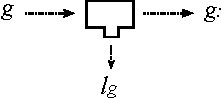
\includegraphics{images/new-label}

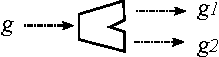
\includegraphics{images/split-gen}


\subsection{Observation Variables}

\begin{eqnarray*}
   s, s' &:& \mathcal S
\\ ls, ls' &:& \mathcal P (Lbl)
\\ g &:& Gen
\\ in, out &:& Lbl
\end{eqnarray*}
We assume a general notion of expressions ($e$)
and say that an expression $e$ is ``ground''
if it's free variables are limited to only $g$, $in$ and $out$.


\subsection{Label-Set Invariants}


We want to distinguish between disjointness only:
\[ \{ in | g | out \} \]
from disjointness with label-set exclusion:
\[ [ in | g | out ] \]

We want to be able to specify that certain combinations
of labels should never appear simultaneously
in the global label set ($ls$).
We do this by defining a label-set invariant $I$
which has alphabet $ls,in,out,g$.

We start by defining a general abstract way of specifying
sets with valid combinations
of values drawn from a parameter type $\tau$.
\RLEQNS{
   i \in I_\tau &::=& \tau   &  \mbox{can contain this value}
\\ &\mid& \otimes(i,\ldots,i) & \mbox{at most one of these allowed to contain}
\\ &\mid& \cup (i,\ldots,i) & \mbox{any of these allowed to contain}
}

We define what it means for an atomic action invocation
to satisfy an invariant parameterised on the label type ($Lbl$).
\RLEQNS{
  ls \textbf{ lsat } I \land A(E|a|N) &\implies& ls' \textbf{ lsat } I
}
We can re-formulate this as a following equivalent test:
\RLEQNS{
   A(E|a|N) \textbf{ sat } I_{Lbl}
   &\defs&
   E \textbf{ lsat } I_{Lbl} \land N \textbf{ lsat } I_{Lbl}
}
In effect we identify the occurrences of labels within this $I$-structure,
and then check the multiplicity constraints:
\RLEQNS{
   L \textbf{ lsat } I_{Lbl} &\defs& res=ok
\\ \textbf{where} && (res,\_) = occChk (occ_L I_{Lbl})
}
The $occ$ function takes a set $L$ of $\tau$ and an $I_\tau$ and returns a $I_\Bool$
that records if the corresponding element of $\tau$ is present in $L$.
\RLEQNS{
   occ &:& \power \tau \fun I_\tau \fun I_\Bool
\\ occ_L~\ell &\defs& \ell \in L
\\ occ_L~\otimes(i_1,\ldots,i_n)
   &\defs&
   \otimes(occ_L~i_1,\ldots,occ_L~i_n)
\\ occ_L~\cup(i_1,\ldots,i_n)
   &\defs&
   \cup(occ_L~i_1,\ldots,occ_L~i_n)
}
The $occChk$ function pattern matches across the boolean values to see if
constraints are satisfied.
The first component of the result is an overall ok/fail indicator,
while the second boolean component indicates if values are present
in any component.
\RLEQNS{
   occChk &:& I_\Bool \fun (\setof{ok,fail}\times \Bool)
\\ occChk(b) &\defs& (ok,b)
\\ occChk(\cup(i_1,\ldots,i_n))
   &\defs&
   (fail,\_),
   \textbf{ if }\exists j @ occChk(i_j) = (fail,\_)
\\ && (ok,b_1 \lor \dots \lor b_n),
   \textbf{ if }\forall j @ occChk(i_j) = (ok,b_j)
\\ occChk(\otimes(i_1,\ldots,i_n))
   &\defs&
   (fail,\_),
   \textbf{ if }\exists j @ occChk(i_j) = (fail,\_)
\\&& (fail,\_) \mbox{ if more than one $(ok,true)$}
\\&& (ok,false) \mbox{ if all are $(ok,false)$}
\\&& (ok,true) \mbox{ if  exactly one $(ok,true)$}
}
We note, as a consequence of the above definitions, that
\RLEQNS{
  \emptyset &  \textbf{lsat} &  I & \elabel{emp-lsat-I}
}
for any label-set invariant $I$.

We introduce a shorthand for invariants illustrated as follows.
\RLEQNS{
  ~ [ a,b,c | d,e | f ]
   &=&
   ls \textbf{ lsat } \otimes(\cup(a,b,c),\cup(d,e),f)
\\ ~[ a | (b|c),(d|e) | f ]
  &=&
  ls \textbf{ lsat } \otimes(a,\cup(\otimes(b,c),\otimes(d,e)),f)
}
In effect we make the involvement of $ls$ implicit,
and use bar ($|$) and comma ($,$) to replace $\otimes$ and $\cup$ respectively.
We also have a shorthand that just denotes
the non-intersecting nature of the arguments.
E.g.,
$\setof{A|B|C}$ asserts that $A$, $B$ and $C$ are mutually disjoint,
without any reference to $ls$ or any other set.

\subsubsection{Invariant Examples}

The following examples show how various instances of $ls \textbf{ lsat } I$
get expanded:
\RLEQNS{
   ~[in|out]
   &=&
   \setof{in} \cap \setof{out} = \emptyset
\\ &\land&
  \setof{in} \subseteq ls \implies \setof{out}\cap ls = \emptyset
\\ &\land&
  \setof{out} \subseteq ls \implies \setof{in}\cap ls = \emptyset
\\
\\ ~[in|\ell|out]
   &=&
   \setof{in} \cap \setof{\ell,out} = \emptyset
\\ &\land&
   \setof{\ell} \cap \setof{in,out} = \emptyset
\\ &\land&
   \setof{out} \cap \setof{in,\ell} = \emptyset
\\ &\land&
  \setof{in} \subseteq ls \implies \setof{\ell,out}\cap ls = \emptyset
\\ &\land&
  \setof{\ell} \subseteq ls \implies \setof{in,out}\cap ls = \emptyset
\\ &\land&
  \setof{out} \subseteq ls \implies \setof{in,\ell}\cap ls = \emptyset
\\
\\ ~[ a | (b|c),(d|e) | f ]
   &=&
   \setof{a} \cap \setof{b,c,d,e,f} = \emptyset
\\ &\land&
   \setof{b,c,d,e} \cap \setof{a,f} = \emptyset
\\ &\land&
   \setof{f} \cap \setof{a,b,c,d} = \emptyset
\\ &\land&
  \setof{a} \subseteq ls \implies \setof{b,c,d,e,f}\cap ls = \emptyset
\\ &\land&
  \setof{b,c,d,e} \subseteq ls \implies \setof{a,f}\cap ls = \emptyset
\\ &\land&
  \setof{f} \subseteq ls \implies \setof{a,b,c,d,e}\cap ls = \emptyset
\\ &\land&
   \setof{b} \cap \setof{c} = \emptyset
\\ &\land&
   \setof{d} \cap \setof{e} = \emptyset
\\ &\land&
  \setof{b} \subseteq ls \implies \setof{c}\cap ls = \emptyset
\\ &\land&
  \setof{c} \subseteq ls \implies \setof{b}\cap ls = \emptyset
\\ &\land&
  \setof{d} \subseteq ls \implies \setof{e}\cap ls = \emptyset
\\ &\land&
  \setof{e} \subseteq ls \implies \setof{d}\cap ls = \emptyset
}
Here one of $b$ or $c$ may occur in $ls$ along with one of  $d$ or $e$.
In this theory,
we use the label generators to ensure that the disjointness
conditions of the invariants are always true, by construction.

\subsubsection{Notation}

\RLEQNS{
   ls(\ell) &\defs& \ell \in ls
\\ ls(L) &\defs& L \subseteq ls
\\ ls(\B\ell) &\defs& \ell \notin ls
\\ ls(\B L) &\defs& L \cap ls = \emptyset
}



\subsection{``Standard'' UTP Predicates}

INTRODUCE

\RLEQNS{
   P \cond C Q
   &\defs&
   C \land P \lor \lnot C \land Q
   & \elabel{UTP-cond-def}
\\ \Skip
   &\defs&
   s'= s \land ls'=ls
   & \elabel{UTP-skip-def}
\\ P \seq Q
   &\defs& \exists s_m,ls_m \bullet
\\ && \qquad P[s_m,ls_m/s',ls'] \land Q[s_m,ls_m/s,ls]
   & \elabel{UTP-seq-def}
\\ C * P
   &=&
   P ; C * P \cond C \Skip
   & \elabel{UTP-loop-unroll}
}
We also define a specialised form of sequential composition
to be used when neither component refers to $ls$ or $ls'$,
and its unit:
\RLEQNS{
   P \seq_s Q
   &\defs&
   \exists s_m \bullet P[s_m/s'] \land Q[s_m/s]
   & \elabel{UTP-s-seq-def}
\\ ii &\defs& s'=s & \elabel{ii-def}
}
Note that if neither predicate mentions $ls$ or $ls'$
then the effect of $\seq$ and $\seq_s$ is the same.
We often omit the $s$ subscript when its use is clear from context.

\subsection{Healthiness Conditions}

\subsubsection{Disjoint Labels}

We have a general healthiness condition (Disjoint Labels) which asserts
that the labels associated with $in$, $out$ and $g$
are different:
\RLEQNS{
  \DL(P) &=& P \land in \neq out \land \setof{in,out} \cap labs(g) = \emptyset
}

\subsubsection{Wheels-within-Wheels}

The key intuition behind this compositional semantics was to take the
$run$ function of the action-system based semantic model used in UTPP,
and drive it inwards to every level of the program.
The original $run$ can be defined in the context of this theory as
\[
  run(P) = ls := \setof{in} ; \lnot (out \in ls) * P
\]
However this failed to keep atomic components ``live''.
They could never be re-executed,
as would be required if they were within an iteration.
Instead it was realised that every construct (atomic and composite)
would have to be within an infinite loop.
\RLEQNS{
   \W(P) &\defs& \true * P &\elabel{W-as-loop}
}
This bold step turns out to be remarkably effective,
with some quite counter-intuitive outcomes.
However it does depend on a specific tweak to the
definition of an atomic action.
In effect we define an atomic action
as placing a basic action inside such a loop,
but within a non-deterministic choice between it
and a \emph{stuttering} step, denoted by UTP skip:
\RLEQNS{
  \catom a &\defs& \W(\Skip \lor A(in|a|out))
}
A result of this is that this stuttering step gets
propagated up to enclosing composites,
so in effect we see $\W(C)=\W(\Skip\lor C)$
where $C$ is any predicate denoting the semantics of a command.
We give more details about this in the section on calculation (\S\ref{sec:calc}).
One key calculational advantage of this is that we can rewrite
the rhs of the definition of $\W$ as:
\RLEQNS{
   \W(P) &  =  & \bigvee_{i \in 0,\dots} \Skip \seq P^i &\elabel{W-as-NDC}
}%
We note explicitly here that, in effect,
our semantic model is based on unbounded non-determinism.

However, for iteration-free programs
we find that there is a finite $k$ such that $P^k = \false$,
in which case the non-determinism is bounded.
We get these finite results that seem very similar
to the results obtained by using $run$ above.
Using $run$ results in predicates that cannot be composed
to get composite behaviour.
However, using $\W$ results in a slight variation,
which is composable!
What turns out to be crucial
to this outcome is the explicit stuttering option in the infinite loop.

\subsubsection{Mumble Closure}

A program's semantics includes all its mumblings,
and so should be unchanged if sequentially composed with itself
using \emph{UTP} sequential composition:
\RLEQNS{
   P \seq P &=& P  & \eref{mumble-closure}
}

\subsection{UTP Denotational Semantics}

INTRODUCE

We present each construct individually,
with full diagrams for each \dots



\subsubsection{Basic Action}

Basic Action $A(E|a|N)$ is enabled when all the labels in $E$
are present in the global label-set
and atomic action $a$ does not evaluate to $\false$
in the current program state.
If so enabled,  it performs action $a$, removes the labels in $E$
from the label-set, and adds in those in $N$.
\RLEQNS{
   A(E|a|N)
   &\defs&
   ls(E) \land a \land ls'=(ls\setminus E) \cup N
   & \elabel{A-def}
}




\newpage
\subsubsection{Atomic Action}


\includegraphics{images/atomic-action}
\RLEQNS{
  \catom a
  &\defs& \DL(\W(\Skip \lor A(in|a|out))) & \elabel{sem:atomic}
\\ &=&  [in|out] \land (\Skip \lor A(in|a|out))
        & \elabel{nf-atomic}
}

Invariant Preservation:
\RLEQNS{
   [in|out]\gamma \land A(in|a|out)\gamma &\implies& [in|out]'\gamma
   & \elabel{atom-inv-ok}
}

\subsubsection{Guarded Atomic Action}
In effect there is no real difference between $c \pgrd a$
and $\true \pgrd (c \land a)$,
so in fact we don't need guarded actions as basic.
This is an advantage of treating the atomic action as a relational predicate
on state.

\RLEQNS{
 c \pgrd a &\defs& \catom{c \land a}  &\elabel{sem:pgrd}
}


\subsubsection{Skip}

\RLEQNS{
   ii     &\defs& s'=s
\\ \cskip &\defs& \catom{ii}  &\elabel{sem:skip}
\\  &=&  [in|out] \land (\Skip \lor A(in|ii|out))
    &\elabel{nf-skip}
}

\newpage
\subsubsection{Sequential Composition}

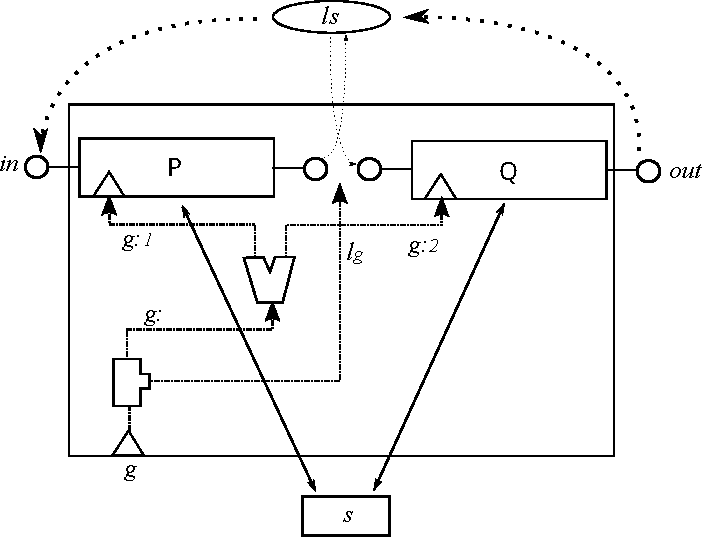
\includegraphics{images/seq-comp-actual}

\RLEQNS{
   P \cseq Q
   &\defs&
   [in|\ell_g|out]\land \W(P[g_{:1},\ell_g/g,out] \lor Q[g_{:2},\ell_g/g,in])
   & \elabel{sem:seq}
}

If $A$ actions in $P$ and $Q$ preserve the invariant,
then so does their composition.
This is immediate by the ground/sound substitution independence
of invariant preservation.



\newpage
\subsubsection{Parallel Composition}

\RLEQNS{
   P \parallel Q
   &\defs&
   [in|(\ell_{g1}|\ell_{g1:}),(\ell_{g2}|\ell_{g2:})|out] \land {}
   & \elabel{sem:par}
\\&& \W(\quad\phlor A(in|ii|\ell_{g1},\ell_{g2})
\\ && \qquad {}\lor
   P[g_{1::},\ell_{g1},\ell_{g1:}/g,in,out]
\\ && \qquad {}\lor
    Q[g_{2::},\ell_{g2},\ell_{g2:}/g,in,out]
\\ && \qquad {}\lor
   A(\ell_{g1:},\ell_{g2:}|ii|out)~)
}


\includegraphics{images/parallel-label-gen}

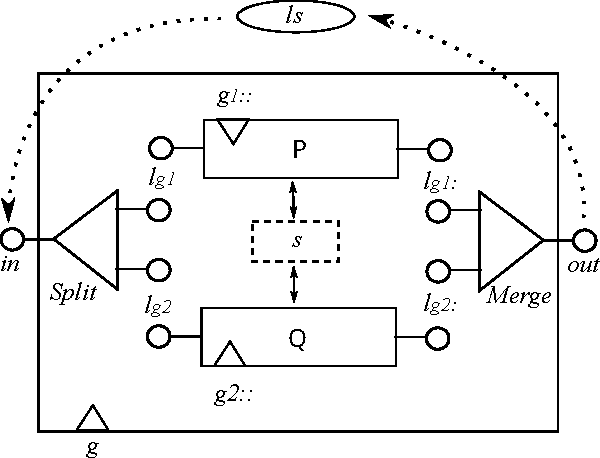
\includegraphics{images/par-comp-actual}


\newpage
\subsubsection{Nondeterministic Choice}

\RLEQNS{
   P + Q
   &\defs&
   [in|\ell_{g1}|\ell_{g2}|out] \land {}
   & \elabel{sem:NDC}
\\ && \W(\quad {}\phlor A(in|ii|\ell_{g1})
\\ && \qquad {} \lor
                     A(in|ii|\ell_{g2})
\\ && \qquad {} \lor
   P[g_{1:},\ell_{g1}/g,in]
\\ && \qquad {} \lor
   Q[g_{2:},\ell_{g2}/g,in]~)
}

\subsubsection{Nondeterministic Loop}


\RLEQNS{
   P^*
   &\defs&
   [in|\ell_g|out] \land {}
   & \elabel{sem:star}
\\ && \W(\quad  \phlor A(in|ii|out)
\\ && \qquad {}\lor A(in|ii|\ell_g)
\\ && \qquad {}\lor P[g_{:},\ell_g,in/g,in,out]~)
}

\newpage
\subsubsection{Conditional Choice}

\RLEQNS{
   P \dcond c Q
   &\defs&
   [in|\ell_{g1}|\ell_{g2}|out] \land {}
   & \elabel{sem:cond}
\\ && \W(\quad {}\phlor A(in|c \land ii|\ell_{g1})
\\ && \qquad {} \lor
                     A(in|\lnot c \land ii|\ell_{g2})
\\ && \qquad {} \lor
   P[g_{1:},\ell_{g1}/g,in]
\\ && \qquad {} \lor
   Q[g_{2:},\ell_{g2}/g,in]~)
}


\includegraphics{images/conditional-actual}

\newpage
\subsubsection{Conditional Loop}


\RLEQNS{
   c \ddo P
   &\defs&
   [in|\ell_g|out] \land {}
   & \elabel{sem:iter}
\\ && \W(\quad  \phlor A(in|\lnot c \land ii|out)
\\ && \qquad {}\lor A(in|c \land ii|\ell_g)
\\ && \qquad {}\lor P[g_{:},\ell_g,in/g,in,out]~)
}


\includegraphics{images/iteration-actual}

\newpage
\subsection{Essential Properties?}

The first key property is that every instance of $A$
in the semantics preserves the invariant.

Looking forward we will want some key algebraic properties:
\RLEQNS{
   ~[S_1|\dots|S_n]
   &=&
   [S_{\rho(1)}|\dots|S_{\rho(n)}]
\\ && \rho \textrm{ a permutation of } 1\dots n
\\ ~[S_1|\dots|S_i|S_{i+1}|\dots|S_n]
   &\implies&
   [S_1|\dots|S_i]
   ,\quad i > 1 &\elabel{I-subsumption}
\\ ~[S_1|\dots|S_n]\gamma &=& [S_1\gamma|\dots|S_n\gamma]
   & \elabel{I-gamma-subst}
\\ A(E|a|N)\gamma &=& A(E\gamma|a|N\gamma)
\\ A(E|a|N) \textbf{ sat } I
   &=&
   A(E|a|N)\gamma \textbf{ sat } I\gamma
   , \quad \mbox{arbitrary }\gamma
\\ ((ls\setminus R)\cup A)(S)
   &=&
   ls(F(R,A,S)) \land P(R,A,S)
\\ \Skip \seq P &=~P~=& P \seq \Skip
\\ (P\seq Q)\gamma &=& P\gamma \seq Q\gamma  & \elabel{seq-gnd-distr}
\\ \Skip\gamma &=& \Skip
\\ \W(P)  && \textrm{monotonic in } P
\\ \W(\W(P)) &=& \W(P) & ?
\\ \W(\W(\Skip \lor P)) &=& \W(\Skip \lor P)
\\ \W(\Skip \lor P) &=& \bigvee_{i \in 0,\dots} \Skip \seq P^i
   & \elabel{W-as-NDC}
\\ \W(P)\gamma &=& \W(P\gamma) & \elabel{W-gamma-subst}
\\ \W(\Skip \lor P) &=& \Skip \lor \W(\Skip \lor P)
\\ I \land \W(P) &=& \W(I \land P) & \elabel{I-W-distr}
}

When $P\gamma$ executes:
\begin{description}
  \item[\elabel{P-removes-in}]
    it will remove $in\gamma$ from $ls$ at some point;
  \item[\elabel{P-removes-g}]
    the only other labels it removes are in $labs(g\gamma)$;
  \item[\elabel{P-adds-out}]
    it adds $out\gamma$ into $ls$ at some point;
  \item[\elabel{P-adds-g}]
    the only other labels it adds are in $labs(g\gamma)$;
  \item[\elabel{P-ignores-rest}]
    and its behaviour is not affected by any label not
    in
    \\$\setof{in\gamma,out\gamma} \cup labs(g\gamma)$.
\end{description}
We can summarise this as follows:
\begin{itemize}
  \item $P\gamma$ actions are enabled by labels in $in\gamma,g\gamma$
  \item $P\gamma$ actions enable actions enabled by $g\gamma,out\gamma$
  \item Remember that the following invariant holds: $[in\gamma|g\gamma|out\gamma]$
\end{itemize}




\newpage
\subsection{Miscellaneous}

Most of this stuff should end up,
if required,
in a Proofs/Justification appendix.

\subsubsection{Semantic Substitutions List}

It can be informative to see the invariants grouped with
the relevant actions and substitutions.
\RLEQNS{
   ~[in|out]
   && A(in|a|out)
\\ && id
\\
\\ ~[in|\ell_g|out]
   && [g_{:1},\ell_g/g,out]
\\ && [g_{:2},\ell_g/g,in]
\\
\\ ~[in|(\ell_{g1}|\ell_{g1:}),(\ell_{g2}|\ell_{g2:})|out]
   && A(in|ii|\ell_{g1},\ell_{g2})
\\ && A(\ell_{g1:},\ell_{g2:}|ii|out)
\\ && [g_{1::},\ell_{g1},\ell_{g1:}/g,in,out]
\\ && [g_{2::},\ell_{g2},\ell_{g2:}/g,in,out]
\\
\\ ~[in|\ell_{g1}|\ell_{g2}|out]
   && A(in|ii|\ell_{g1})
\\ && A(in|ii|\ell_{g2})
\\ && [g_{1:},\ell_{g1}/g,in]
\\ && [g_{2:},\ell_{g2}/g,in]
\\
\\ ~[in|\ell_g|out]
   && A(in|ii|out)
\\ && A(in|ii|\ell_g)
\\ && P[g_{:},\ell_g,in/g,in,out]
\\
\\ ~[in|\ell_{g1}|\ell_{g2}|out]
   && A(in|c \land ii|\ell_{g1})
\\ && A(in|\lnot c \land ii|\ell_{g2})
\\ && [g_{1:},\ell_{g1}/g,in]
\\ && [g_{2:},\ell_{g2}/g,in]
\\
\\ ~[in|\ell_g|out]
\\ && A(in|\lnot c \land ii|out)
\\ && A(in|c \land ii|\ell_g)
\\ && [g_{:},\ell_g,in/g,in,out]
}

\subsubsection{Nested Invariants}

For each composite,
we show how its component substitutions affect their invariants
and any entailment relationships that arise.
We don't show the conditional variants of choice and iteration
because their invariants and substitutions are the same as those
in the corresponding non-deterministic constructs.

Semantics Reminder:
\RLEQNS{
  \catom a
  &\defs& [in|out] \land \W(\Skip \lor A(in|a|out))
\\ P \cseq Q
   &\defs&
   [in|\ell_g|out]\land \W(P[g_{:1},\ell_g/g,out] \lor Q[g_{:2},\ell_g/g,in])
\\ P \parallel Q
   &\defs&
   [in|(\ell_{g1}|\ell_{g1:}),(\ell_{g2}|\ell_{g2:})|out] \land {}
\\&& \W(\quad\phlor A(in|ii|\ell_{g1},\ell_{g2})
\\ && \qquad {}\lor
   P[g_{1::},\ell_{g1},\ell_{g1:}/g,in,out]
\\ && \qquad {}\lor
    Q[g_{2::},\ell_{g2},\ell_{g2:}/g,in,out]
\\ && \qquad {}\lor
   A(\ell_{g1:},\ell_{g2:}|ii|out)~)
\\ P + Q
   &\defs&
   [in|\ell_{g1}|\ell_{g2}|out] \land {}
\\ && \W(\quad {}\phlor A(in|ii|\ell_{g1})
\\ && \qquad {} \lor
                     A(in|ii|\ell_{g2})
\\ && \qquad {} \lor
   P[g_{1:},\ell_{g1}/g,in]
\\ && \qquad {} \lor
   Q[g_{2:},\ell_{g2}/g,in]~)
\\ P^*
   &\defs&
   [in|\ell_g|out] \land {}
\\ && \W(\quad  \phlor A(in|ii|out)
\\ && \qquad {}\lor A(in|ii|\ell_g)
\\ && \qquad {}\lor P[g_{:},\ell_g,in/g,in,out]~)
}


\paragraph{Sequential Composition}

\begin{description}
  \item[Invariant]
    $[in|\ell_g|out]$
  \item[Substitutions]
    $[g_{:1},\ell_g/g,out]$ and $[g_{:2},\ell_g/g,in]$
  \item[Component Invariants]
    $$\begin{array}{|l|c|c|}
    \hline
      \mbox{Type} & \mbox{as }P & \mbox{as }Q
    \\\hline
      \catom\_ & [in|\ell_g] & [\ell_g|out]
    \\\hline
       \_\cseq\_& [in|\ell_{g:1}|\ell_g] & [\ell_g|\ell_{g:2}|out]
    \\\hline
       \_\parallel\_
       & [in|(\ell_{g:11}|\ell_{g:11:}),(\ell_{g:12}|\ell_{g:12:})|\ell_g]
       & [\ell_g|(\ell_{g:21}|\ell_{g:21:}),(\ell_{g:22}|\ell_{g:22:})|out]
    \\\hline
    \end{array}$$
\end{description}
Hmmm \dots, no simple relationship is emerging.

\section{Semantic Calculations}\label{sec:calc}

\textbf{SHOULD COMPUTE PARTIAL NORMAL FORMS
FOR COMPOSTITES}

\subsection{Composing $A$s}\label{ssec:comp-A}

We have a problem in that actions defined using $A(\dots)$
are not closed under standard UTP sequential composition (\eref{UTP-seq-def}).
We need a more general form,
where the labels removed are not necessarily
exactly those that had to be present to enable the action.
We call this eXtended atomic action $X$ and it is defined as follows:
\RLEQNS{
   X(E|a|R|A)
   &\defs&
   ls(E) \land s' \in \sem a s \land ls' = (ls \setminus R) \cup A
   & \elabel{X-def}
}
We can then re-define $A$ in terms of $X$:
\RLEQNS{
   A(E|a|N)
   &=&
   X(E|a|E|N)
   & \elabel{A-alt-def}
}
The key law is one regarding sequentially composing $X$s:
\RLEQNS{
   \lefteqn{X(E_1|a|R_1|A_1) ; X(E_2|b|R_2|A_2)} &&& \elabel{X-then-X}
\\ &=& (E_2\setminus A_1) \cap R_1 = \emptyset
\\ &\land&
   X(E_1 \cup (E_2\setminus A_1)
       |a\seq b
       |R_1 \cup R_2
       |(A_1 \setminus R_2) \cup  A_2)
}
The condition $(E_2\setminus A_1) \cap R_1 = \emptyset$
characterises all those cases were the second $X$ is enabled
immediately after the first $X$ terminates
(i.e., without any outside interference).

\textbf{ANOTHER IMPORTANT LAW:}
If $(E_1 \cup N_1) \cap (E_2 \cup N_2)$, then
\[
  A(E_1|a|N_1) \seq A(E_2|b|N_2)
  =
  A(E_1\cup E_2|a\seq b|N_1\cup N_2)
\]
(and vice-versa)!

\subsection{Normal Form}\label{sec:normal-form}

All the semantics above have an invariant $I_P$,
zero or more atomic actions ($A_i$),
plus zero or more language sub-component predicates ($P_j$)
assembled into a predicate of the form:
\[
  I_P
  \land
  \W( A_1 \lor \dots \lor A_m
     \lor
     P_1\sigma_1 \lor \dots \lor P_n\sigma_n )
\]
where each $\sigma_i = [G_i,I_i,O_i/g,in,out]$,
with all $G_i$, $I_i$ and $O_i$ being ground
and satisfying the invariant $[I_i|labs(G_i)|O_i]$.

\subsubsection{Stuttering Propagates Up}

We show that for any predicate $P$ resulting from the
semantics applied to a program,
that the stuttering on such a predicate propagates up:
\RLEQNS{
   P &=& \Skip \lor P
}



\subsubsection{Nondeterministic Iteration}

Given that we have,
for predicates $P$ used in program semantic definitions,
that
\[
  \W(P) = \bigvee_{i \in 0\dots} \Skip \seq P^i
\]
we find that the following outcomes result:
\begin{enumerate}
  \item
    Every program $P$ can be transformed,
    in principle at least,
    to the form
    \[
      I_P \land \Skip
      \lor
      \bigvee_{n \in 0\dots}  (I_P \land I_n \land X(E_n|a_n|R_n|A_n) \land S_n)
    \]
    for suitable choices of $I_n$, $E_n$, $a_n$, $R_n$, $A_n$ and $S_n$,
    depending on $P$.
    In particular, we find that the $E_n$ and $A_n$ all satisfy the relevant
    label-set invariants.
  \item
    For any complete program that does not use iteration constructs,
    this expansion is finite.
  \item
    For any complete program the $S_n$
    term in $X(E_n|a_n|R_n|A_n) \land S_n$
    is a ground-expression, and is statically decidable as $\true$ or $\false$.
    If $\true$, we find that the above term
    can be be simplified to one of the form $A(E_n|a_n|A_n)$.
    We do not prove this, but note that we have observed it as a result
    of test calculations and these lead us to believe it is true in general.
\end{enumerate}
\RLEQNS{
   P
   &=&
   I_P \land \Skip
      \lor
      \bigvee_{n \in 0\dots}
      (I_P \land I_n \land X(E_n|a_n|R_n|A_n) \land S_n)
   & \elabel{UTCP-NF}
}
This can be shown by an inductive argument over the language syntax,
noting that the sequential composition of two such forms
can itself be transformed into such a form.
In effect this defines a \emph{normal form} for our semantics.


An important law we shall require is that the UTP sequential
composition of two normal forms can itself be expressed
as such a normal form:
\RLEQNS{
   I \land (\Skip\lor\bigvee A_i) \seq J \land (\Skip\lor\bigvee B_j)
   &=&
   I \land J \land (\Skip\lor\bigvee (A_i \seq B_j))
   &\elabel{nf-seq}
}
This is an easy result of the fact that $\seq$ distributes through $\lor$,
and $\Skip$ is a unit for it as well.


\subsection{Normal Form Results for Atomic components}

We now present the results of calculations of normal forms for every language
construct, given atomic sub-components,
and the generic case.

For ease of reading in the former,
we display the invariant $I$ on the first line,
followed by the list of $A(\dots)$ disjuncts, perhaps several on a line,
as follows
\RLEQNS{
   res &=& I
\\ && A(E_1|a_1|N_1) \quad A(E_1|a_2|N_2)) \quad \dots
}
We omit parentheses, logical operators, and the ever-present $\Skip$.
In general we try to put all the single atomic steps on the first line,
with all the mumblings on lower lines.
Here we also just write $a$ instead of $\catom a$,
for brevity.

In the latter generic case we  \emph{\dots to be determined \dots}

\subsubsection{Atomic Actions}
\RLEQNS{
   a &=& [in|out]
\\ && A(in|a|out) & \elabel{NF:atomic-a}
\\
\\ \cskip &=& [in|out]
\\ && A(in|ii|out) & \elabel{NF-skip}
}

\subsubsection{Sequential Composition}

With atomic components:
\RLEQNS{
   a \cseq b
   &=& [in|\ell_g|out]
\\ && A(in|a|\ell_g)\quad  A(\ell_g|b|out)
\\ && A(in|a\seq b|out)
}

With generic components:
\RLEQNS{
   P \cseq Q
   &=& [in|\ell_g|out]
\\ && A(in|a|\ell_g)\quad  A(\ell_g|b|out)
\\ && A(in|a\seq b|out)
}


\subsubsection{Non-deterministic Choice}
\RLEQNS{
   a + b
   &=& [in|\ell_{g1}|\ell_{g2}|out]
\\ &&  A(in|ii|\ell_{g1}) \quad A(in|ii|\ell_{g2})
       \quad
       A(\ell_{g1}|a|out) \quad A(\ell_{g2}|b|out)
\\&& A(in|a|out) \quad A(in|b|out)
}


\subsubsection{Parallel Composition}
Here $\#n$ denotes mumblings of length $n$.
\RLEQNS{
   a \parallel b
   &=& [in\mid([\ell_{g1}|\ell_{g1:}],[\ell_{g2}|\ell_{g2:}])\mid out]
\\ &&  A(in|ii|\ell_{g1},\ell_{g2})
       \quad
       A(\ell_{g1:},\ell_{g2:}|ii|out)
       \quad
       A(\ell_{g1}|a|\ell_{g1:})
       \quad
       A(\ell_{g2}|b|\ell_{g2:}) &
\\ && A(in|a|\ell_{g1:},\ell_{g2})
      \quad
      A(\ell_{g1},\ell_{g2}|b;a|\ell_{g1:},\ell_{g2:})
      \quad
      A(in|b|\ell_{g2:},\ell_{g1}) & \#2
\\ && A(\ell_{g1},\ell_{g2}|a ; b|\ell_{g1:},\ell_{g2:})
      \quad
      A(\ell_{g2:},\ell_{g1}|a|out)
      \quad
      A(\ell_{g1:},\ell_{g2}|b|out) & \#2
\\ && A(in|b;a|\ell_{g1:},\ell_{g2:})
      \quad
      A(in|a;b|\ell_{g1:},\ell_{g2:}) & \#3
\\ && A(\ell_{g1},\ell_{g2}|b;a|out)
      \quad
      A(\ell_{g1},\ell_{g2}|a;b|out) & \#3
\\ && A(in|b;a|out)
      \quad
      A(in|a;b|out) & \#4
}

\subsubsection{Non-deterministic Iteration}
The actions that denote a terminating
run with zero or more complete iterations
are \textbf{emboldended} below.
\RLEQNS{
   a^*
   &=& [in|\ell_g|out]
\\ &&  \mathbf{A(in|ii|out)} \quad A(in|ii|\ell_g) \quad A(\ell_g|a|in)
\\ &&  A(\ell_g|a|out) \quad A(\ell_g|a|\ell_g) \quad A(in|a|in)         &\#2
\\ &&  \mathbf{A(in|a|out)} \quad A(in|a|\ell_g) \quad A(\ell_g|a^2|in)  &\#3
\\ &&  A(\ell_g|a^2|out) \quad A(\ell_g|a^2|\ell_g) \quad A(in|a^2|in)   &\#4
\\ &&  \mathbf{A(in|a^2|out)} \quad A(in|a^2|\ell_g) \quad A(\ell_g|a^3|in) &\#5
\\ &&  A(\ell_g|a^3|out) \quad A(\ell_g|a^3|\ell_g) \quad A(in|a^3|in) &\#6
\\ && \vdots & \#7\dots
}
An obvious recurrent pattern (based on mumbling depth) has emerged:
\RLEQNS{
   &&  \mathbf{A(in|a^n|out)} \quad A(in|a^n|\ell_g) \quad A(\ell_g|a^{n+1}|in) &\#2n+1
\\ &&  A(\ell_g|a^{n+1}|out) \quad A(\ell_g|a^{n+1}|\ell_g) \quad A(in|a^{n+1}|in) &\#2n+2
}
We can also identify a pattern based on number of $a$s performed:
\RLEQNS{
   \alpha_0 && \mathbf{A(in|ii|out)} \quad A(in|ii|\ell_g)
\\ \alpha_1 && A(\ell_g|a|in) \quad A(\ell_g|a|out) \quad A(\ell_g|a|\ell_g) \quad A(in|a|in)
\\          && \mathbf{A(in|a|out)} \quad A(in|a|\ell_g)
\\ \alpha_2 && A(\ell_g|a^2|in) \quad A(\ell_g|a^2|out) \quad A(\ell_g|a^2|\ell_g) \quad A(in|a^2|in)
\\          && \mathbf{A(in|a^2|out)} \quad A(in|a^2|\ell_g)
\\
\\ \alpha_n && A(\ell_g|a^n|in) \quad A(\ell_g|a^n|out) \quad A(\ell_g|a^n|\ell_g) \quad A(in|a^n|in)
\\          && \mathbf{A(in|a^n|out)} \quad A(in|a^n|\ell_g)
}


\newpage
\subsection{Essential Properties?}

\RLEQNS{
   X(E|a|R|A)\gamma &=& X(E\gamma|a|R\gamma|A\gamma)
   & \elabel{X-gnd-subs}
\\ (\bigvee_n X_n)^2
   &=& \bigvee_{n_1,n_2} X_{n_1} \seq X_{n_2}
   & \elabel{NF-squared}
\\ (\bigvee_p Y_p \lor \bigvee_q Z_q)^2
     &=& \bigvee_{p_1,p_2}  (Y_{p_1} \seq Y_{p_2})
\\&\lor& \bigvee_{q_1,q_2}  (Z_{q_1} \seq Z_{q_2})
\\&\lor& \bigvee_{p,q}  (Y_p \seq Z_q)
\\&\lor& \bigvee_{q,p}  (Z_q \seq Y_p)
  & \elabel{NF+NF-squared}
\\ &=& \bigvee_r X_r,\textrm{ for appropriate } r
  & \elabel{NF-squared-alt}
\\ (\bigvee_p Y_p \lor \bigvee_q Z_q)^n
     &=& \bigvee_r X_r,\textrm{ for appropriate } r
  & \elabel{NF-powered}
\\ \W(\Skip \lor \bigvee_p Y_p \lor \bigvee_q Z_q)
     &=& \bigvee_r X_r,\textrm{ for appropriate } r
  & \elabel{W-of-NDC-is-NF}
}
Add in X-then-X and related properties.

Nice to have:
the combined invariants ensure that the normal form
has the form:
\[
  P = \bigvee_n A(E_n|a_n|N+n)  \qquad \elabel{NF-only-As}
\]
Is this the case?

\subsubsection{STOP PRESS! $P^2=P$ ?}

The semantics of a program $P$
contains a stuttering step $\Skip$,
all the single atomic actions $A(\dots)$,
and all the feasible mumblings
$X(\dots) = A(\dots) \seq A(\dots) \seq \dots \seq A(\dots)$.
Calculations for law $\cskip\cseq P = P$ suggest the following conjecture:
\begin{center}
\fbox{$\large P \seq P = P \qquad \elabel{mumble-closure}$}
\end{center}
This is because combining elements of $P$ with each other results
in either infeasibility, or some other already present mumble.
\newpage
\subsection{Miscellaneous}

More stuff for proofs section.


We shall first demonstrate that the stuttering $\Skip$
introduced in the atomic action semantics
propagates up into the program composites,
so that, for example, we could have defined sequential composition
as:
\RLEQNS{
   P \cseq Q
   &\defs&
   [in|\ell_g|out]\land
   \W(\Skip \lor P[g_{:1},\ell_g/g,out] \lor Q[g_{:2},\ell_g/g,in])
   & \elabel{sem:seq-alt}
}
We argue by induction over program syntax.

What we shall demonstrate is that, for all commands $C$
with a definition $C = \W(P)$, for $P$ related to $C$ as appropriate,
that the following predicates are all equal:
\RLEQNS{
  \W(\Skip \lor P) \quad = & \W(P)& = \quad \Skip \lor \W(P)
 & \elabel{W-prog-stutters}
}
The base case is easy, here $c$ is $\catom a$,
and $P$ is $\Skip \lor A(in|a|out)$:
\RLEQNS{
  && \W(\Skip \lor (\Skip \lor A(in|a|out)))
\EQ{$\lor$-assoc, $\lor$-idem}
\\&& \W(\Skip \lor A(in|a|out))
\EQ{\eref{sem:atomic}}
\\&& \catom a
}
For the inductive step we assume the hypothesis
for command $C$ and its semantics predicate  $C = \W(P)$,
that:
\RLEQNS{
   \W(P) &=& \W(\Skip \lor P) &\elabel{hyp:P-stutters}
}
We now make use of the following deduction:
\RLEQNS{
  && \W(\Skip \lor Q)
\EQ{loop unrolling}
\\&& (\Skip\lor Q)\seq(\Skip\lor Q)\seq(\Skip\lor Q)\seq(\Skip\lor Q)\seq\dots
\EQ{$\lor$-$\seq$-distr, diagonalisation, removing identical terms}
\\&& \bigvee_{i \in \Nat} \Skip\seq Q^i & \elabel{W-stutter-is-NDC}
}
An immediate consequence of this is that
\RLEQNS{
  \W(\Skip \lor Q) &=& \Skip \lor \W(\Skip\lor Q) & \elabel{W-exposes-II}
}
We now show that the same holds for a composite $F(C,\ldots)$
that directly includes $P$, or rather its semantics $C$
, along with some other stuff.
Inspection of all the semantic definitions reveals
that the form of the semantics of $F$ is the following,
where $\sigma$ is a ground substitution:
\RLEQNS{
   F(C,\ldots) &=& \W(C\sigma \lor \ldots)
}
We now can easily show that we get stuttering here also:
\RLEQNS{
  && \W(C\sigma \lor \dots)
\EQ{$C$ is meaning of $P$}
\\&& \W(\W(P)\sigma \lor \dots)
\EQ{\eref{hyp:P-stutters}}
\\&& \W(\W(\Skip \lor P)\sigma \lor \dots)
\EQ{\eref{W-exposes-II}}
\\&& \W((\Skip\lor\W(\Skip \lor P))\sigma \lor \dots)
\EQ{substitution}
\\&& \W(\Skip\sigma\lor\W(\Skip \lor P)\sigma \lor \dots)
\EQ{Lemma $\Skip\sigma=\Skip$}
\\&& \W(\Skip\lor\W(\Skip \lor P)\sigma \lor \dots)
\EQ{reverse first two steps above}
\\&& \W(\Skip\lor C\sigma \lor \dots)
}

\appendix
\section{Root}\label{ha:Root}

We do a quick run-down of the Commands\cite{conf/popl/Dinsdale-YoungBGPY13}.

\subsection{Syntax}

\def\Atm#1{\langle#1\rangle}
\def\rr#1{r{\scriptstyle{#1}}}

\begin{eqnarray*}
   a &\in& \Atom
\\ C &::=&
 \Atm a \mid \cskip \mid C \cseq C \mid C+C \mid C \parallel C \mid C^*
\\ g &:& Gen
\\ \ell &:& Lbl
\\ G &::=&  g \mid G_{:} \mid G_1 \mid G_2
\\ L &::=& \ell_G
\end{eqnarray*}


\subsection{Domains}


\subsubsection{Rooted Paths}

This Root file is a re-work of the Views semantics
replacing label generators by ``rooted'' label-paths.

We start by defining three basic ways to transform a rooted path:
``step'' ($:$);
``split-one'' ($1$);
and ``split-two'' ($2$).
\RLEQNS{
   S &\defs& \setof{:,1,2}
}

We now define a rooted path as an expression of the form
of the variable $r$ followed by zero or more $S$ transforms.
\RLEQNS{
   \sigma,\varsigma &\defs& S^*
\\ R &::=& r | R S
\\   & = & r\sigma
}
These have to be expressions as we shall want to substitute for $r$
in them.

\subsubsection{Path Ordering}
\RLEQNS{
   R &\le& R\sigma
\\ R1\sigma &<& R\!:\!\varsigma
\\ R2\sigma &<& R\!:\!\varsigma
}
\RLEQNS{
   r &\le& r\sigma
}
\RLEQNS{
   R1\sigma &<& R\!:\!\varsigma
}
\RLEQNS{
   R2\sigma &<& R\!:\!\varsigma
}
\RLEQNS{
   R &\le& R\sigma
}

\subsection{Shorthands}

We support a shorthand (that views a set as its own collection
of corresponding $n$-ary characteristic functions)
that denotes $x \in S$ by $S(x)$ and $ X \subseteq S$ by $S(X)$,
and omits $\{$ and $\}$ from around enumerations when context makes
it clear a set is expected

\begin{eqnarray*}
   ls(\ell) &\defs& \ell \in ls
\\ ls(L) &\defs& L \subseteq ls
\\ ls(\B\ell) &\defs& \ell \notin ls
\\ ls(\B L) &\defs& L \cap ls = \emptyset
\end{eqnarray*}


\paragraph{Set Swapping}

We update a set by removing some elements
and replacing them with new ones:
\RLEQNS{
   A \ominus (B,C) &\defs& (A \setminus B) \cup C
}

\subsection{Alphabet}

\begin{eqnarray*}
   s, s' &:& \mathcal S
\\ ls, ls' &:& \mathcal P (R)
\\ r &:& R
\end{eqnarray*}

We define our dictionary alphabet entries,
and also declare that the predicate variables $a$, $b$ and $c$
will refer to atomic state-changes,
and so only have alphabet $\setof{s,s'}$.

\subsection{``Standard'' UTP Constructs}

\begin{eqnarray*}
   P \cond c Q
   &\defs&
   c \land P \lor \lnot c \land Q
\\ P ; Q
   &\defs&
   \exists s_m,ls_m \bullet P[s_m,ls_m/s',ls'] \land Q[s_m,ls_m/s,ls]
\\ c * P
   &=&
   P ; c * P \cond c \Skip
\end{eqnarray*}

We need to update some definitions from standard UTP as follows:

\paragraph{Updating UTP Skip ($\Skip$)}\label{hd:updating-UTP-II}

We know have a concrete definition for $\Skip$,
as well as a known alphabet.
\RLEQNS{
   \Skip &=& ls'=ls \land s'=s
\\ \alpha \Skip &=& \setof{ls,ls',s,s'}
}

\subsection{WwW Basic Shorthands}

Atomic actions have a basic behaviour that is described by
\[
ls(E) \land s' \in \sem a s \land ls' = (ls\setminus E) \cup N
\]
where $E$ is the set of necessary enabling labels,
$a$ is a relation over shared state,
and $N$ is the set of new labels deposited upon completion.
We shall abstract the above as
\[
A(E|a|N)
\]
There is a slightly more general form that removes labels
that may differ from those doing the enabling:
\[
ls(E) \land s' \in \sem a s \land ls' = (ls\setminus R) \cup A
\]
where $R$ and $A$ are sets of labels respectively removed, then added
on the action is complete.
We abstract this as
\[
  X(E|a|R|A)
\]
and note that
\[
  A(E|a|N) = X(E|a|E|N).
\]


\subsubsection{Generic Atomic Behaviour}

\begin{eqnarray*}
   X(E|ss'|R|A)
   &\defs&
   ls(E) \land [ss'] \land ls'=(ls\setminus R)\cup A
\end{eqnarray*}

We do want the following simplification:
\begin{eqnarray*}
  X(E|a|E|N) &=& A(E|a|N)
\end{eqnarray*}

\begin{eqnarray*}
   A(E|ss'|N)
   &\defs&
   X(E|ss'|E|N)
\end{eqnarray*}


\subsubsection{Coding Label-Set Invariants}

We have a key invariant as part of the healthiness
condition associated with every semantic predicate,
namely that the labels $r$ and $\rr:$ never occur in  $ls$ at
the same time:
\[
 ( r \in ls \implies \rr: \notin ls )
 \land
 ( \rr: \in ls \implies r \notin ls )
\]
This is the Label Exclusivity invariant.

Given the way we shall use substitution of $r$ by
other rooted paths, for sub-components,
we shall see that we will get a number of instances of this.
We adopt a shorthand notation,
so that the above invariant is simply
\[
  [r|\rr:]
\]
So we define the following general shorthand:
\RLEQNS{
   ~[L_1|L_2|\dots|L_n]
   &\defs&
   \forall_{i,j \in 1\dots n}
    @
    i \neq j \implies
     ( L_i \cap ls \neq \emptyset \implies L_j \cap ls = \emptyset )
\\ \multicolumn{3}{c}{\elabel{short-lbl-exclusive}}
}
What needs to be kept in mind regarding this shorthand notation
is that $ls$ is mentioned under the hood,
and it is really all about what can be present in the global label-set
at any instant in time.


Now, we need to define invariant satisfaction.
Our invariant applies to $A$ and $X$ atomic actions:
\RLEQNS{
   A(E|a|N) \textbf{ sat } I
   &\defs&
   E \textbf{ lsat } I \land N \textbf{ lsat } I
\\ X(E|a|R|A)  \textbf{ sat } I
   &\defs&
   E \textbf{ lsat } I \land A \textbf{ lsat } I
}

Now we have to define \textbf{lsat}:
\RLEQNS{
   \textbf{lsat}_S [L_1|\dots|L_n]
   &\defs&
   \#(filter ~\textbf{lsat'}_S \seqof{L_1,\ldots,L_n}) < 2
\\ \textbf{lsat'}_S \setof{\ell_1,\dots,\ell_n}
  &\defs&
  \exists i @ \textbf{lsat''}_S \ell_i
\\ \textbf{lsat''}_S \ell &\defs& \ell \in S
}

\subsubsection{Invariant Trimming}

We can use the invariant to trim removal sets,
given an enabling label or label-set.
\RLEQNS{
   I \textbf{ invTrims } X(E|a|E,L|A)
   &\defs&
   \lnot(\setof{E,L} \textbf{ lsat } I)
}

\subsubsection{Wheels within Wheels}\label{hc:WwW}

The wheels-within-wheels healthiness condition
insists that $r$ and $\rr:$ are never simultaneously in
the label-set $ls$,
and that our semantic predicates are closed under mumbling.
\RLEQNS{
   \W(C)
   &\defs&
   [r|\rr:] \land \left(~\bigvee_{i\in 0\dots} C^i~\right)
\\ ii &\defs& s'=s
}

Unrolling $\W(C)$, using $I$ for $[r|\rr:]$,
and noting that
$
\bigvee_{i \in \Nat} C^i
= \Skip \lor (C\seq\bigvee_{i \in \Nat} C^i)
$.
\RLEQNS{
   \W(C) &=& I \land \bigvee C^i
\\ &=& I \land (\Skip \lor C\seq\bigvee C^i)
\\ &=& I \land (\Skip \lor C\seq((\Skip \lor C\seq\bigvee C^i)))
\\ &=& I \land (\Skip \lor C \lor C^2\seq\bigvee C^i)
\\ &=& I \land (\Skip \lor C \lor C^2\seq((\Skip \lor C\seq\bigvee C^i)))
\\ &=& I \land (\Skip \lor C \lor C^2 \lor C^3\seq\bigvee C^i)
\\ &\vdots&
\\ &=& I \land (\Skip \lor C \lor \dots C^{k-1} \lor C^k\seq\bigvee C^i)
\\ &=& I \land (~(\bigvee_{i < k} C^i) \lor (\bigvee_{i \geq k} C^i)~)
}
We assume $\seq$ binds tighter than $\lor$.

\subsection{WwW Semantic Definitions}

The definitions, using the new shorthands:
\RLEQNS{
   \W(C) &\defs& [r|\rr:]
                 \land
                 \left(\bigvee_{i\in 0\dots} C^i\right)
\\ ii &\defs& s'=s
\\
\\ \Atm a &\defs&\W(A(r|a|\rr:))
\\
\\ \cskip
   &\defs&
   \Atm{ii}
}
The following are all under review (they lack sufficient invariants).
\RLEQNS{
   C \cseq D
   &\defs&
   \W(~    A(r|ii|\rr1)
      \lor C[\rr1/r]
      \lor A(\rr{1:}|ii|\rr2)
      \lor D[\rr2/r]
      \lor A(\rr{2:}|ii|\rr:) ~)
\\
\\ C + D
   &\defs&
   \W(\quad {}\phlor A(r|ii|\rr1) \lor A(r|ii|\rr2)
\\ && \qquad {} \lor
   C[\rr1/r] \lor D[\rr2/r]
\\ && \qquad {} \lor A(\rr{1:}|ii|\rr:) \lor A(\rr{2:}|ii|\rr:) ~)
\\
\\ C \parallel D
   &\defs&
   \W(\quad\phlor A(r|ii|\rr1,\rr2)
\\ && \qquad {}\lor
   C[\rr1/r]
   \lor D[\rr2/r]
\\ && \qquad {}\lor
   A(\rr{1:},\rr{2:}|ii|\rr:)~)
\\
\\ C^*
   &\defs&
   \W(\quad  \phlor A(r|ii|\rr1) \lor A(\rr1|ii|\rr:)
\\ && \qquad {}\lor C[\rr1/r]    \lor A(\rr{1:}|ii|\rr1) ~)
}

\subsubsection{Coding Atomic Semantics}

\RLEQNS{
   \Atm a &\defs&\W(A(r|a|\rr:))
}

\newpage
\subsubsection{Coding Skip}

\RLEQNS{
   ii &\defs& s'=s
\\ \cskip
   &\defs&
   \Atm{ii}
}


\subsubsection{Coding Sequential Composition}

\RLEQNS{
   C \cseq D
   &\defs& [r|\rr1|\rr{1:}|\rr2|\rr{2:}|\rr:] \land {}
\\ && \W(\quad {}\phlor A(r|ii|\rr1)
\\ && \qquad {} \lor C[\rr1/r]
\\ && \qquad {} \lor A(\rr{1:}|ii|\rr2)
\\ && \qquad {} \lor D[\rr2/r]
\\ && \qquad {} \lor A(\rr{2:}|ii|\rr:)~)
}

\subsubsection{Coding (Non-Det.) Choice}

\RLEQNS{
   C + D
   &\defs& [r|\rr1|\rr{1:}|\rr2|\rr{2:}|\rr:] \land {}
\\&& \W(\quad {}\phlor A(r|ii|\rr1) \lor A(r|ii|\rr2)
\\ && \qquad {} \lor
   C[\rr1/r] \lor D[\rr2/r]
\\ && \qquad {} \lor A(\rr{1:}|ii|\rr:) \lor A(\rr{2:}|ii|\rr:) ~)
}

\subsubsection{Coding Parallel Composition}

\RLEQNS{
   C \parallel D
   &\defs& ~
   [r|\rr1,\rr2,\rr{1:},\rr{2:}|\rr:] \land
   [\rr1|\rr{1:}] \land
   [\rr2|\rr{2:}] \land {}
\\&& \W(\quad\phlor A(r|ii|\rr1,\rr2)
\\ && \qquad {}\lor
   C[\rr1/r]
   \lor D[\rr2/r]
\\ && \qquad {}\lor
   A(\rr{1:},\rr{2:}|ii|\rr:)~)
}

\subsubsection{Coding Iteration}

\RLEQNS{
   C^*
   &\defs& [r|\rr2|\rr1|\rr{1:}|\rr:] \land {}
\\&& \W(\quad  \phlor A(r|ii|\rr2)
\\ && \qquad {}\lor A(\rr2|ii|\rr1)
               \lor C[\rr1/r]
               \lor A(\rr{1:}|ii|\rr2)
\\ && \qquad {}\lor A(\rr2|ii|\rr:) ~)
}


\subsection{Reductions for WWW}\label{hb:WWW-reduce}

\subsubsection{Recognisers for WWW}\label{hc:v-recog}

\RLEQNS{
   ls'=ls\ominus(S_1,S_2)
   &\rightsquigarrow&
   \seqof{S_1,S_2}
   & \ecite{sswap-$;$-prop.}
}

\paragraph{$A$ then $A$}

\RLEQNS{
  && A(E_1|a|N_1) \seq A(E_2|b|N_2)
\EQ{proof in Views.tex }
\\&& X(E_1 \cup (E_2\setminus N_1)
       |a\seq b
       |E_1 \cup E_2
       |N_1 \setminus E_2 \cup  N_2)
       \land (E_2\setminus N_1) \cap E_1 = \emptyset
}

\paragraph{$X$ then $A$}

\RLEQNS{
  && X(E_1|a|R_1|A_1) \seq A(E_2|b|N_2)
\EQ{proof in Views.tex }
\\&& X(E_1 \cup (E_2\setminus A_1)
       |a\seq b
       |R_1 \cup E_2
       |A_1 \setminus E_2 \cup  N_2)
       \land (E_2\setminus A_1) \cap R_1 = \emptyset
}

\paragraph{$A$ then $X$}

\RLEQNS{
  && A(E_1|a|N_1) \seq X(E_2|b|R_2|A_2)
\EQ{proof in Views.tex}
\\&& X(E_1 \cup (E_2 \setminus N_1)
      | a\seq b
      | E_1 \cup R_2
      | N_1 \setminus R_2 \cup A_2)
     \land
     (E_2 \setminus N_1) \cap E_1 = \emptyset
}

\paragraph{$X$ then $X$}

\RLEQNS{
  && X(E_1|a|R_1|A_1) \seq X(E_2|b|R_2|A_2)
\EQ{proof in Views.tex }
\\&& X(E_1 \cup (E_2\setminus A_1)
       |a\seq b
       |R_1 \cup R_2
       |A_1 \setminus R_2 \cup  A_2)
       \land (E_2\setminus A_1) \cap R_1 = \emptyset
}

\paragraph{$I$ collapses $X$ to $A$}
\RLEQNS{
   \lnot(\setof{E,L} \textbf{ lsat } I)
   &\implies&  X(E|a|E,L|N) = A(E|a|N)
}
Given $I$ and $X(E|a|R|A)$, we proceed as follows:
\begin{enumerate}
  \item Let $D = R \setminus E$
  \item Compute
    $D' =
       \setof{  d | d \in D,
                    \lnot (E\cup\setof d \textbf{ lsat } I)}
    $
  \item
    If $D = D'$ then return $A(E|a|A)$
  \item
    Else, return $X(E|a|E\cup(D \setminus D')|A)$.
\end{enumerate}

\paragraph{General Stuff}~

If $a$ and $b$ have alphabet $\setof{s,s'}$,
then
$(a \seq b)[G,L,M/g,in,out) = a\seq b$.

\subsection{Loop Unrolling for Views}\label{hb:WWW-unroll}

Iteration  satisfies the loop-unrolling law:
\[
  c * P  \quad=\quad (P ; c * P ) \cond c \Skip
\]
But we also support several styles and degrees of unrolling:
\begin{eqnarray*}
   c*P
   &=_0& (P\seq c*P) \cond c \Skip
\\ &=_1& \lnot c \land \Skip
         \lor
         c \land P ; c * P
\\ &=_2& \lnot c \land \Skip
         \lor
         c \land P ; \lnot c \land \Skip
         \lor
         c \land P ; c \land P ; c * P
\\ &=_3& \lnot c \land \Skip
         \lor
         c \land P ; \lnot c \land \Skip
         \lor
         c \land P ; c \land P ; \lnot c \land \Skip
         \lor
         c \land P ; c \land P ; c \land P ; c *P
\\ && \vdots
\\ &=_n& \left(
           \bigvee_{i=0}^{n-1}  (c \land P)^i \seq \lnot c \land \Skip
         \right)
         \lor
         (c \land P)^n \seq c *P
\end{eqnarray*}


\subsection{Calculation Results}

Given the idiom $\true * (\Skip \lor Q)$
we look for pre-computed $Q$-cores,
noting that our final semantics will have the form
\[
  I \land ( \Skip \lor Q \lor Q^2 \lor \dots Q^k)
\]
where $I$ is the label-set invariant
and $Q^i = \false$ for all $i > k$.

When we change from:
\RLEQNS{
   \W(C) &\defs& \true * (\Skip \lor C)
\\ \Atm a &\defs&\W(A(in|a|out)) \land [in|out]
}
\noindent
to:
\RLEQNS{
   \W(C) &\defs& \true * C
\\ \Atm a &\defs&\W(\Skip \lor A(in|a|out)) \land [in|out]
}
\noindent
the calculation outcomes
for \texttt{athenb}, \texttt{aorb}, \texttt{awithb} and \texttt{itera} are unchanged,
and consequently so are all the other calculations.



\bibliographystyle{splncs03}
\bibliography{UTCP-SBMF2017-MAIN}

\end{document}
